\documentclass[11pt]{article}

\usepackage{graphicx}
\usepackage[dvipsnames]{color}
\usepackage[hidelinks]{hyperref}
\usepackage[numbers]{natbib}
%pPara poder modificar los margenes
\usepackage{vmargin}
%Para usar el español
\usepackage[spanish]{babel}
\usepackage[utf8]{inputenc}
\begin{document}
%Portada
\setpapersize{A4}

%Indice
\tableofcontents
\newpage

\section{Creación de formularios}
Una vez adaptada la base de datos de no relacional a relacional y creados los correspondientes correspondientes operaciones CRUD de las tablas, hemos pasado a la creación o a la adaptación de los formularios con los nuevos datos que les corresponde a cada uno de ellos. Para ello, tuvimos que aprender y experimentar con Angular JS, framework de javascript, que requiere un vasto conocimiento para el desarrollo de los formularios y de los archivos para el correcto funcionamiento de estos. 
\subsection{Formulario de registro de usuarios}
El primer formulario que tuvimos que tratar fue el registro de usuarios, siendo este el punto de inicio para los posteriores formularios a crear.\\\\
En el TFG de David ya venía un registro implementado con sus correspondientes campos, pero al probar la aplicación habíamos encontrado algunos errores que tuvimos que corregir. Uno de los errores que encontramos era que permitía introducir una contraseña no robusta de cualquier longitud y sin ninguna restricción. De manera que la hemos hecho más robusta con una longitud mínima de 8 caracteres, mínimo una mayúscula, mínimo una minúscula y mínimo un carácter especial. También el campo email no verificaba si era un email correcto, de modo que tuvimos que crear las validaciones correspondientes por si no contenía el “@” o el “.” .\\\\
 En el formulario de David existían dos campos para la contraseña: contraseña y repetir contraseña, donde ambos campos deben contener el mismo contenido para que se pueda permitir la validación del formulario y la creación del usuario, en cambio al pedir la contraseña repetida si se introducía una contraseña distinta al campo de “contraseña “ lo aceptaba y se procedía a proceso de registro. Por eso tuvimos que añadir la validación y los mensajes de error correspondientes para que no se permita el registro si los dos campos no son iguales.\\\\
Una vez arreglados los errores, añadido las mejoras y las nuevas validaciones del registro tuvimos que añadir los campos nuevos correspondientes a cada tipo de usuario de la base de datos. \\\\
En el formulario de registro se permite la elección de tres tipos de usuarios externos: profesor externo, estudiante externo, entidad.\\\\
Para la entidad aparte de los campos ya existentes en el formulario se añadió un nuevo campo “nombre entidad” que representa el nombre de la entidad principal que creará el formulario.\\\\
En el caso del estudiante externo no se han añadido nuevos campos en el formulario, pero si el cambio de funcionalidad del campo universidad. Antes en el campo universidad se permitía introducir un texto, pero como eso podía llegar a causar incoherencias en la base de datos puesto que cualquier usuario podría introducir una universidad que no existiese o con algún carácter incorrecto por lo cual se decidió cambiar. De modo que el campo universidad se convirtió en una lista desplegable que permite una única selección por el estudiante de entre ochenta y tres universidades a elegir.  No se permite la validación del registro si no se selecciona alguna universidad de la lista. \\\\
Para el profesor externo se añadió un campo nuevo y se cambiaron las funcionalidades de algunos otros campos. El campo “universidad” tenía el mismo problema que en el caso anterior por lo que se produjo el mismo cambio. Además, tuvimos que introducir un nuevo campo "Área/s de conocimiento" que representa las áreas de conocimiento que tiene el profesor externo a registrar. Este campo es un desplegable que permite la selección múltiple de entre las ciento noventa áreas disponibles que guardamos en la base de datos en la tabla "area conocimiento". Se puede seleccionar entre una o varias áreas de conocimiento y en el caso de que se haya cometido un error al seleccionar un área se permite desmarcar la elección, pero no se permite la validación del registro en el caso de que no se haya seleccionado ningún área de conocimiento de la lista.\\\\

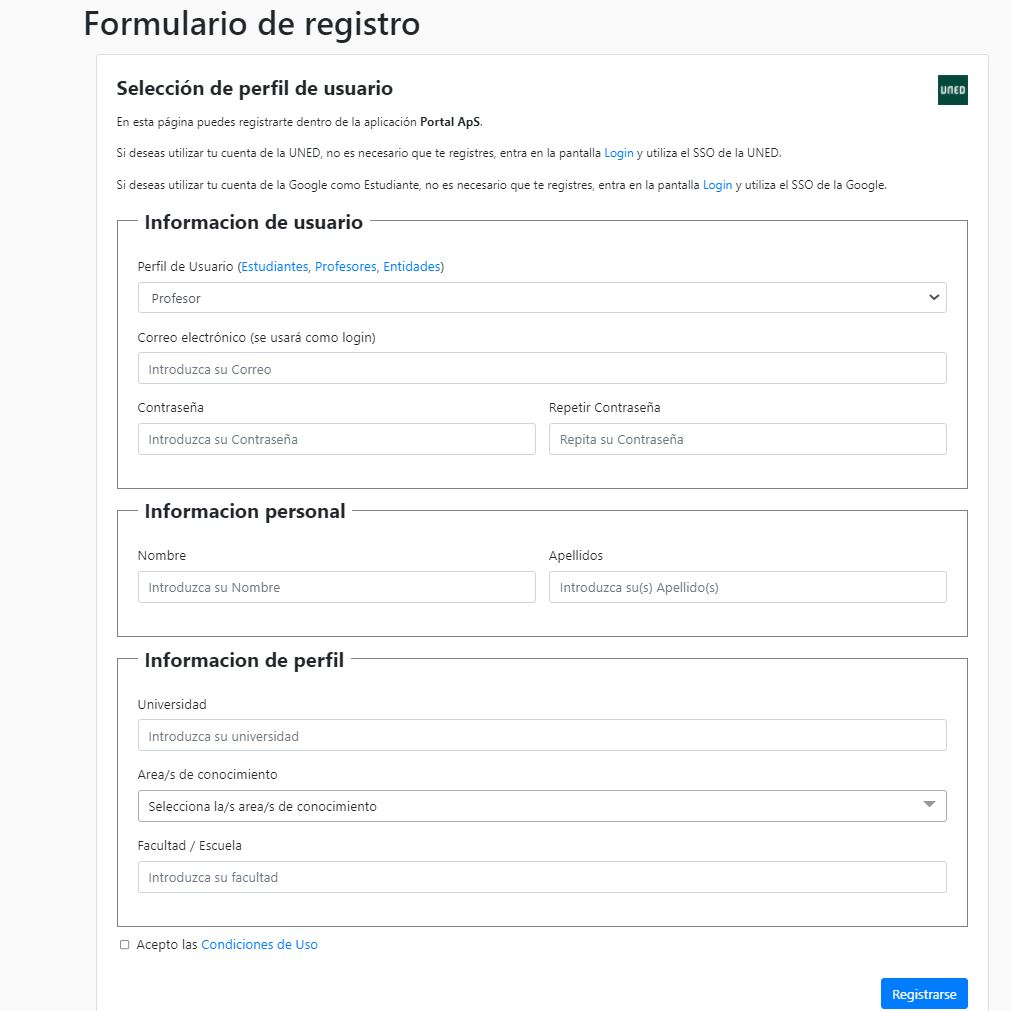
\includegraphics[width=\textwidth]{registro}
\\\\

\subsection{Formulario para editar los datos de un usuario}
En el TFG de David ya existía un formulario para la edición de los datos de un usuario con sus correspondientes campos, pero al cambiar el tipo de base de datos y al introducir nuevos datos en algunos de los tipos de usuarios tuvimos que adaptarlo. \\\\
También añadimos validaciones para los campos como email, contraseña y repetir contraseña. Para el campo email se permitía emails incorrectos sin el “@” o sin el “.” , la contraseña se permitía no robusta y al introducir la contraseña repetida permitía que no fuera igual a lo introducido en el campo contraseña. Una vez añadidas las validaciones se introdujeron los campos necesarios para el formulario en función del tipo de usuario.
Para la entidad a parte de los campos ya existentes en el formulario se añadió el campo “nombre entidad” que representa el nombre de la entidad principal que creará el formulario. Dicho campo viene con el valor ya rellenado, teniendo la posibilidad de cambiar su valor.\\\\
Para el estudiante externo no se han añadido nuevos campos en el formulario, pero si el cambio de funcionalidad del campo universidad, que se convirtió en un desplegable que permite una única selección por el estudiante de una lista de ochenta y tres universidades a elegir.  No se permite la validación de registro si no se selecciona alguna universidad de la lista. El campo  viene con el valor ya relleno, teniendo la posibilidad de cambiar su valor.\\\\
En el caso del profesor externo se añadió un campo nuevo y cambiaron la funcionalidad de algunos otros campos más. El campo universidad cambió de ser un texto introducido por el usuario a ser una lista con las universidades para así no llegar a causar incoherencias en la base de datos. El campo ya viene relleno y se puede cambiar su valor por cualquiera de la lista disponible. Además tuvimos que introducir un nuevo campo “Área/s de conocimiento” que representa las áreas de conocimiento de un profesor. Se puede seleccionar al menos una área de servicio y el valor viene ya relleno con los valores del usuario ya creado.


\subsection{Formulario creación demanda de servicio}
Para poder crear una demanda de servicio en la base de datos que nos permita ejecutar el algoritmo de matching tuvimos que crear el formulario desde cero con sus correspondientes archivos puesto que en el anterior TFG no existía.\\\\
Para ello se tuvo que crear su correspondiente modelo con los campos necesarios para la creación de la demanda:id, titulo, descripcion, imagen, ciudad, objetivo, área de servicio, inicio del periodo de definición, final del periodo de definición, inicio del periodo de ejecución, final del periodo de ejecución, fecha fin, observaciones temporales, necesidad social, titulación local, creador, comunidad beneficiaria, createdAt y updatedAt.\\\\
El creador es la entidad que está conectada en la aplicación y la cual accede a la creación de la demanda de servicio.
Para el formulario de la creación de la demanda de servicio se han creado las validaciones correspondientes para los campos a completar de manera que no se pueda permitir la creación de la demanda si alguno de ellos no es correcto y los mensajes correspondientes a los errores.\\\\
En función del campo se permiten distintos valores acorde a los campos que les corresponden de la base de datos: \\
\begin{itemize} 
	\item Los campos título, descripción, imagen,ciudad,objetivo, necesidad social, comunidad beneficiaria, observaciones temporales permiten introducir texto. 
	\item  Los campos periodoDefinicionIni, periodoDefinicionFin, periodoEjecucionIni, periodoEjecucionFin, fechaFin permiten un valor de tipo fecha.
	\item El campo Área/s de servicio es un desplegable que permite selección múltiple entre un total de setenta y ocho áreas de servicios disponibles en la base de datos en la tabla "area servicio" En el caso de que se haya seleccionado algún área de servicio por error se puede descartar la selección. Hay que seleccionar por lo menos una opción para que se pueda validar el campo correctamente.
\end{itemize}
Una vez completados o seleccionados los campos a completar se comprueba el formulario, y en el caso de que estén todos los campos correctos se valida el formulario y se crea la oferta de servicio insertándose en la base de datos. En caso contrario, se avisa al usuario que los campos no están completados adecuadamente para que este proceda a su corrección.\\\\


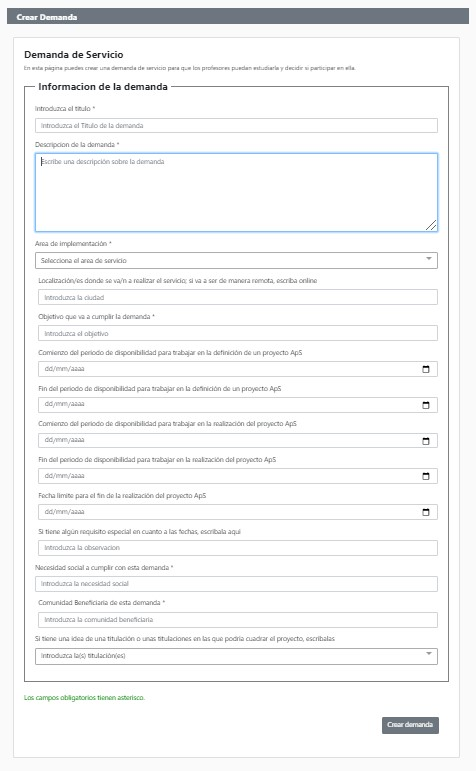
\includegraphics[width=\textwidth]{demanda}
\\\\

\subsection{Formulario creación oferta de servicio}
Para poder crear una oferta de servicio que sirva para el proceso de matching tuvimos que crear el formulario de creación de una oferta de servicio.En el anterior TFG no existía el formulario, así que tuvimos que crearlo desde cero con sus correspondientes archivos para el correcto funcionamiento en angular js.\\\\
Para ello se tuvo que crear su correspondiente modelo con los campos necesarios para la creación de la oferta: id, titulo, descripcion, imagen, created at, updated at, cuatrimestre, año académico, fecha límite, observaciones, creador, área servicio, asignatura objetivo y profesores. El creador es el profesor interno que está conectado en la aplicación y el cual accede a la creación de la oferta de servicio.\\\\
Para el formulario de la creación de la oferta de servicio se han creado las validaciones correspondientes para los campos a completar de manera que no se pueda permitir la creación de la oferta si alguno de ellos no está correcto y los mensajes correspondientes a los errores. \\\\
En función del campo se permiten distintos valores acorde a los campos que les corresponden de la base de datos: \\
\begin{itemize} 
	\item En los campos título, descripción, asignatura, observaciones temporales se permite introducir texto.
	\item En los campos año académico se permite un valor de tipo numérico que represente un año válido.
	\item El campo fecha límite permite un valor de tipo fecha. 
	\item  El campo cuatrimestre es un desplegable que permite una sola elección entre: Primer cuatrimestre, segundo cuatrimestre y anual. Hay que seleccionar una opción para que se pueda validar el campo correctamente.
	\item El campo Área/s de servicio es un desplegable que permite selección múltiple entre un total de setenta y ocho áreas de servicios disponibles en la base de datos en la tabla “area servicio” En el caso de que se haya seleccionado algún área de servicio por error se puede descartar la selección. Hay que seleccionar por lo menos una opción para que se pueda validar el campo correctamente.
\end{itemize}
Una vez rellenos todos los campos del formulario se procede a su validación, en el caso de estar correcto se almacena la oferta de servicio en la base de datos, en caso contrario se notificará al usuario para que complete de manera correcta los campos erróneos.


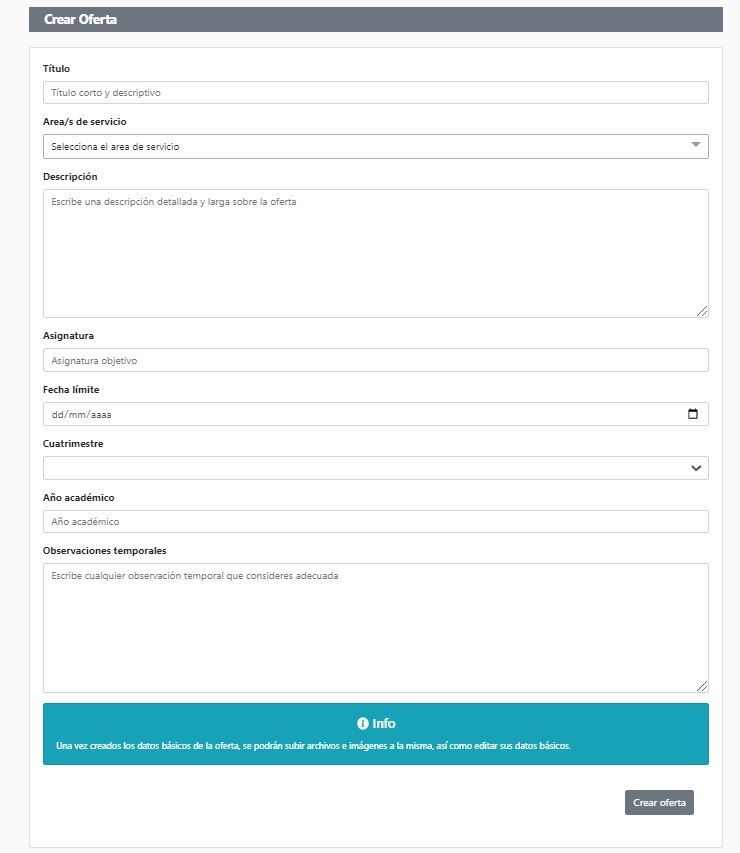
\includegraphics[width=\textwidth]{oferta}
\\\\

\subsection{ Formulario creación de partenariado profesor}
Una vez creados los formularios de oferta de servicio y demanda de servicio hemos procedido al desarrollo del formulario para la creación del partenariado de un profesor.
El formulario para la creación del partenariado del profesor no existía en el anterior TFG, así que se procedió a su creación desde cero. Para ello, tuvimos que crear los archivos y el modelo necesarios para el formulario. El formulario aparece con unos campos ya rellenos, algunos de los cuales son editables. Se necesitan los datos de la oferta y la demanda en cuestión para poder realizar la creación del formulario.\\\\
En la creación del formulario de partenariado del profesor los datos de la demanda de servicio de la entidad beneficiaria vienen ya completados y sin posibilidad de editarlos En cambio, los datos de la oferta hechos por el profesor responsable que procede a la creación del formulario si tiene la posibilidad de cambiar los datos. Estos datos vienen rellenados con los datos de la demanda de servicio.\\\\
El formulario está dividido en tres partes para la distinción entre los datos generales del partenariado que serán la combinación de los datos en común o los datos más relevantes del formulario, los datos de la oferta y los datos de la demanda. También hemos creado validaciones para todos los campos del formulario, para que no se permitan campos vacíos.\\\\
En el formulario el título y la descripción son una  combinación de los títulos y descripciones de la oferta y la demanda, estos campos son editables. Los datos de la demanda de servicio vienen rellenadas, pero no son editables:  las áreas de servicio,la entidad de la demanda, la localización de desarrollo del partenariado, la finalidad, la comunidad beneficiaria, las fechas, asignatura objetivo, titulaciones locales, cuatrimestre y año académico. Aparece como profesor responsable, el de la oferta, siendo un campo editable que se da a elegir entre una lista de todos los profesores internos de la base de datos.\\\\
 El campo equipo de profesores es una lista que da la posibilidad de selección múltiple y viene ya rellenada con los valores de la oferta de servicio ya creada. El profesor que procede a la creación del formulario elige si se aceptan personas externas. El área de servicio de la oferta no es un campo editable. Para que se pueda validar el formulario no deben existir campos vacíos o mal completados, y se mostrarán los mensajes para que informe al usuario de los campos a cambiar o completar. Una vez completado correctamente, al aceptarlo se pasa del estado EN\_NEGOCIACION a EN\_CREACION. Si se rechaza pasa al estado SUSPENDIDO.
 \\\\
 
 
 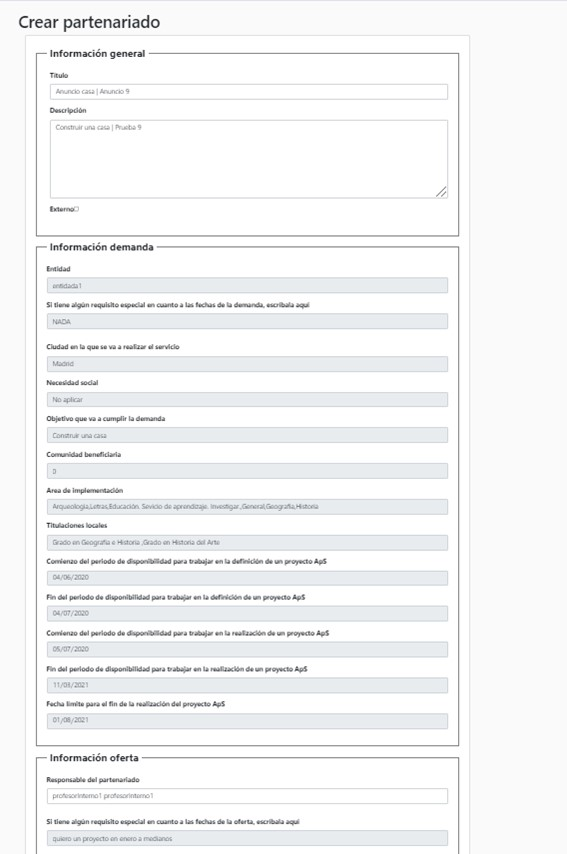
\includegraphics[width=\textwidth]{partenariado1}
 \\\\

 
 
 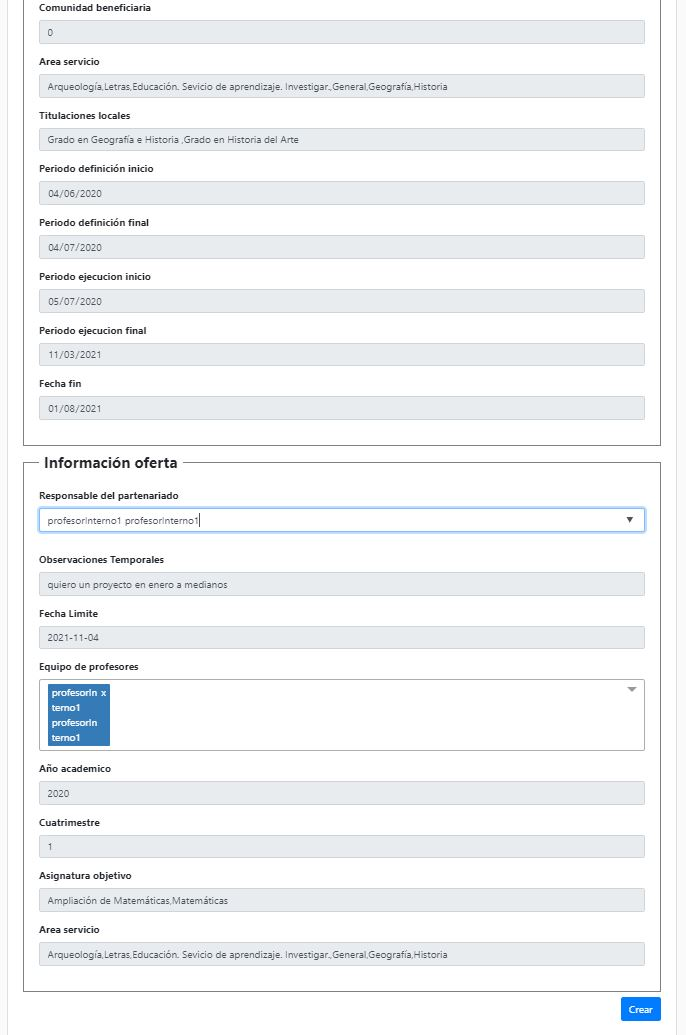
\includegraphics[width=\textwidth]{partenariado2}
 \\\\
 
 \section{Matching entre oferta de servicio y demanda de servicio}
 
 \subsection{Definición del matching }

 Para nuestro TFG hemos implementado un algoritmo de matching para las ofertas y las demandas, de manera que cogiendo una oferta y una demanda de la base de datos verificamos si se puede realizar una negociación entre ellas a partir de la información que contiene cada una. Partiendo de unas especificaciones del algoritmo que se estableció entre nosotros y los tutores del TFG, las hemos aplicado para poder obtener la información relacionada representada por un porcentaje, con el cual  se decidirá el resultado final.  Cuantos más datos haya relacionados entre una oferta y una demanda, más porcentaje sacará nuestro algoritmo. El objetivo del algoritmo de matching es ayudar a los profesores a encontrar más fácilmente demandas relacionadas a sus propuestas y a las entidades a obtener ofertas acorde a sus solicitudes. \\\\
 
 Definimos el matching según nuestro algoritmo, como el proceso que consiste en identificar los datos que se ajustan a unos criterios de coincidencia los cuales se van a enumerar a continuación en los siguientes párrafos. De modo que si se encuentran suficientes puntos de similitud entre los datos recopilados, estos son considerados para sacar un porcentaje de coincidencia, donde si este es menor que el valor mínimo establecido no se considerará matching. El valor mínimo que hemos establecido para nuestro algoritmo para considerar la existencia de un matching es 50\%.
 \\\\
 
  \subsection{Criterios de matching y anti matching}
 \subsubsection{Criterios de matching }
  
 Hemos definido unos criterios en base a los datos proporcionados por los usuarios en las ofertas y demandas de servicio según los cuales se resolverá el matching:
 
 \begin{itemize} 	
 	\item Hacer coincidir las descripciones tanto de la oferta como de la demanda de servicio mediante Procesamiento del Lenguaje Natural (NLP).
 Para ello hemos tenido que buscar las palabras comunes del idioma español y almacenarlas en un fichero, para así poder  procesarlas para obtener el resultado deseado. El procedimiento consiste en dadas las dos descripciones, las guardamos en dos estructuras simples de datos, quitamos las palabras comunes (aquellas que sean iguales a las del fichero) y nos quedamos con las que puedan coincidir en las dos descripciones, cada una de estas se guarda en una estructura simple de datos. Al tenerlas, empezamos a procesar las palabras resultantes de las dos descripciones, distinguiendo las mayúsculas, minúsculas, tildes y caracteres especiales, donde obtenemos el número de palabras que coinciden de las descripciones. Para poder obtener el porcentaje de coincidencias, dividimos el número de palabras coincidentes con la descripción que tiene el menor número de palabras. Dicho porcentaje se tendrá en cuenta para poder calcular el matching final.
 
 	\item Encontrar la similitud entre las áreas de servicio tanto de la oferta como de la demanda. Se dispone de setenta y ocho áreas de servicio en la base de datos para poder realizar esta comprobación. Para ello se comparan todas las áreas de servicio de ambas, y se devuelve el número de coincidencias. Cuanto mayor dicho número, mayor probabilidad de que se produzca el matching.
 
 	\item Obtener las coincidencias entre las titulaciones elegidas por la entidad a la hora de introducir la demanda (si es que ha introducido algunas) con las titulaciones en las que imparten docencia los profesores asociados a la oferta. 
 Se dispone de ciento nueve titulaciones locales en la base de datos para poder realizar esta comprobación. Tanto la oferta como la demanda pueden tener una o varias titulaciones, y en función de la cantidad de titulaciones de la demanda se calcula el resultado el cual será un porcentaje obtenido a partir de la división del número total de titulaciones que producen coincidencias entre el  número total de las titulaciones de la demanda.
 
 	\item Obtener las coincidencias en las observaciones temporales de la oferta de servicio y de la demanda de servicio que hemos aplicado mediante Procesamiento del Lenguaje Natural (NLP). Una vez obtenidas las dos observaciones temporales tanto de la oferta como de la demanda, procedemos a aplicar el algoritmo para emparejar las palabras que coinciden de los dos lados y obtener un porcentaje. Para ello una vez más se quitan las palabras comunes de las descripciones y se guardan las palabras no comunes para cada una de las observaciones en una estructura de datos. Tras esto, se procesan cada una de las estructuras, resultando el número de observaciones temporales que coinciden. El porcentaje de coincidencias se obtiene mediante la división del número de palabras coincidentes entre el valor (observaciones temporales) que tiene el menor número de palabras.
 
 	\item Relacionar el área de servicio de la demanda y las titulaciones en las que imparte docencia los profesores que participan en la oferta. Para ello tenemos asignamos al menos una titulación a cada área de servicio, estas relaciones están almacenadas en la tabla “matching\_areaservicio\_titulacion” de la base de datos. De esta manera se podrá sacar la relación directa o indirecta entre estos dos valores para así poder calcular un porcentaje válido para el resultado final de nuestro algoritmo de matching. Por ejemplo el área de servicio "Computer\_science" se relacionaría con las titulaciones "Ingeniería de Computadores", "Ingeniería Informática", “Ingeniería del Software”, "Telecomunicación", etc. Para el cálculo del porcentaje se usa el mismo procedimiento que en los demás criterios, contamos el número de coincidencias y lo dividimos entre la cantidad total de las áreas de servicio.
 
 	\item Encontrar la similitud entre el área de servicio de la demanda y las áreas de conocimiento UNESCO de los profesores que participan en la oferta. Para ello tenemos asignamos al menos un área de conocimiento a cada área de servicio, estas relaciones están almacenadas en la tabla “matching\_areas” de la base de datos. Se dispone de ciento noventa áreas de conocimiento en la base de datos para poder realizar esta comprobación. Para ello tenemos en cuenta las áreas de conocimiento con las cuales están relacionadas las áreas de servicio de la demanda y de la oferta como el principal valor en el cálculo del porcentaje. Para encontrar las posibles coincidencias contamos el número de ellas y lo dividimos entre las áreas de servicio de las demanda.
  \end{itemize}
 
 \subsubsection{Criterios de anti matching }
 
 También hemos definido unos criterios de anti matching para encontrar posibles incompatibilidades entre los datos proporcionados.\\\\
 Para poder realizar el anti matching nos hemos centrado en los valores temporales tanto de la demanda como de la oferta. Para lo cual hemos partido de si el periodo de definición inicial de la demanda no está fuera de la fecha de finalización de la oferta. En el caso de que esté fuera del plazo se considera anti matching y se descartará la posibilidad de una negociación entre dicha demanda y oferta. \\\\
 
 En el caso de que los plazos estén en el periodo aceptado, se procede a verificar si el año académico establecido para empezar dicha colaboración en la oferta coincide con el año de ejecución establecido de la demanda. Si no coinciden, se considera anti matching y en caso contrario se continúa con la comprobación de los siguientes valores temporales.\\\\
 
 Otro criterio de anti matching es mirar si el periodo de ejecución de la demanda encaja en el periodo de duración del cuatrimestre o los cuatrimestres elegidos y el año académico. De tal manera que si no se corresponden correctamente, se considera incompatibilidad y se descarta la negociación. Hemos considerado que en los meses de verano no se puedan realizar negociaciones entre la oferta y la demanda y cualquier comprobación de matching será descartada si los valores temporales coinciden con este periodo.\\\\
 
 
  \subsection{Matching definitivo}

 Una vez obtenidos todos los porcentajes de los criterios de matching y los resultados del anti matching procedemos a averiguar si se produce el match definitivo, para ello multiplicamos cada uno de los porcentajes anteriormente mencionados por los valores que les corresponden a cada uno definidos en el fichero configuracion.txt y son sumados para obtener el valor de compatibilidad entre la oferta y la demanda. El fichero configuracion.txt almacena en cada línea datos como “pesoFechas = 0.3”, “pesoTitulaciones = 0.3”, “pesoAreaServicio = 0.2”...  \\\\
 
 Si el valor obtenido es mayor que 0.5 se considerará un match definitivo y se almacenará en la base de datos en un tabla que contendrá el porcentaje final, el id de la oferta, el id de la demanda y un atributo booleano, “procesado”, que se pone a true indicando si paso por el proceso de verificación del match. La tabla de matching de la base de datos contendrá la información sobre los posibles match y no match de entre las demandas y ofertas procesadas, de esta manera la aplicación del algoritmo de matching se ejecuta una única vez por cada pareja oferta-demanda. \\\\
 
 A partir de un matching de una oferta de servicio y una demanda se crea un partenariado. Para ello primero, el profesor responsable de la oferta acepta el match y rellena el formulario que tiene  algunos campos rellenados automáticamente a partir de información contenida en la oferta o en la demanda, lo que conlleva la creación de un partenariado en estado “en creación” y el envío de una notificación a la entidad. Después, la entidad podría aceptar el match, rellenando un segundo formulario, teniendo algunos campos rellenados automáticamente a partir de información contenida en la oferta o en la demanda, lo que provocaría que el partenariado pasará al estado “en negociación” \\\\
 
  \subsection{Ejemplo de matching}
  
   A continuación se muestra un ejemplo válido de matching con una oferta y una demanda dada, con un porcentaje de matching mayor del 50\%. Se expondrá la aplicación de cada uno de los criterios de matching y anti matching, y cómo se llegó al resultado final del algoritmo, de modo que se irá paso a paso por cada etapa del algoritmo que hemos creado.\\\\
  Dada una oferta con los datos más significativos para el matching:\\
  \begin{itemize} 
  	\item descripción: “ Proyecto de investigacion en biologia y tecnologia”
  	\item observaciones temporales : “Me interesa que se empiece en septiembre”
  	\item área servicio: “Biologia, Tecnologia digital, inteligencia artificial”
  	\item  area conocimiento: “Biologia celular”
  	\item titulaciones: “Grado en Ciencias Ambientales”
  	\item cuatrimestre : Primer cuatrimestre
  	\item  fecha límite: 2022/03/ 04
  	\\
  \end{itemize}
  Y una demanda con los datos:\\
  \begin{itemize} 
  	\item titulaciones: “Grado en Ciencias Ambientales”
  	\item descripción: “ Proyecto de investigacion en biologia”
  	\item observaciones temporales : “En septiembre 2022”
  	\item área servicio: “Biologia”
    \item inicio de periodo de definición: 2021/09/04
    \item final de periodo de definición : 2021/09/07
    \item inicio de periodo de ejecución 2021/09/14
    \item final de periodo de ejecución: 2022/03/03
    \item fecha fin: 2022/03/04
  \end{itemize}

  Empezamos a buscar las coincidencias mediante NLP entre las dos descripciones, quitamos las palabras comunes de ambas y nos quedamos con las no comunes. La descripción de la oferta se queda en “Proyecto,investigacion,biologia,tecnologia” y la de la demanda se queda en “proyecto,investigacion,biologia”. Sacamos el porcentaje resultante entre el número de coincidencias que es tres y la longitud total de la descripción con menos valores que es tres, por lo que se consigue el máximo de coincidencias entre las dos descripciones. El mismo procedimiento se aplica también para las observaciones temporales, donde el número de coincidencias resultante es 1 y el total de valores de la menor de las observaciones es 2, por lo que el resultado tras ello es 50\% de coincidencias. Se buscan las coincidencias entre ambas áreas de servicios, entre ambas  titulaciones y entre las áreas de servicio y las áreas de conocimiento donde tras ello resulta un porcentaje alto para el matching, dado que comparten áreas de servicio, titulaciones y hay un número elevado de coincidencias entre las áreas de servicio y las áreas de conocimiento.\\\\
  Tras ello se comprueban las observaciones temporales para saber si se produce un ati matching.\\\\
  Primero se verifica si la fecha de inicio de definición del periodo es mayor que la fecha límite definida en la oferta, en este caso se pasa al siguiente comprobación ya que la fecha límite de la oferta es superior. También se verifican si las otras fechas cuadran entre ellas, para así poder verificar si se podrán ejecutar ambas en el primer cuatrimestre. \\\\
  Tras ello, una vez obtenidos todos los resultados, cada una se multiplica por su correspondiente peso para ver si se produce el matching. Como se puede observar, tras el número elevado de coincidencias, se produce el matching entre la oferta y la demanda y por lo consecuente se inserta la relación en la tabla “matching”.\\\\
  

\end{document}